
% Beamer Presentation

\documentclass{beamer}
\mode<presentation> {
% Theme
\usetheme{metropolis}
%\setbeamertemplate{footline} % To remove the footer line in all slides uncomment this line
%\setbeamertemplate{footline}[page number] % To replace the footer line in all slides with a simple slide count uncomment this line
%\setbeamertemplate{navigation symbols}{} % To remove the navigation symbols from the bottom of all slides uncomment this line
}

%Packages
\usepackage{pdfcomment}
\newcommand{\pdfnote}[1]{\marginnote{\pdfcomment[icon=note]{#1}}}
\usepackage{graphicx} % Allows including images
\usepackage{booktabs} % Allows the use of \toprule, \midrule and \bottomrule in tables
%\usepackage{cite}
\usepackage[numbers]{natbib} % For bibliography
\usepackage{multirow}
\usepackage{hyperref}
%\usetheme{Warsaw}
\usepackage[absolute,overlay]{textpos}
\usepackage{xcolor}


% Colors
%\definecolor{Red}{rgb}{0.7,0,0}
%\definecolor{Blue}{rgb}{0,0,0.8}

% Prepare title and TOC
\title[Short title]{Introduction to R} 
\author{Marco Chiapello} 
\institute[Center for Proteomics] 
{
Center for Proteomics\\
University of Cambridge \\ 
\medskip
\textit{mc983@cam.ac.uk} 
}
\date{06-07/07/2016} 

%\AtBeginSection[]
%{
%\begin{frame}<beamer>
%\frametitle{Overview}
%\tableofcontents[currentsection]
%\end{frame}
%}


%-------------------------------------------
% MAIN DOCUMENT
%-------------------------------------------
\usepackage{Sweave}
\begin{document}
\Sconcordance{concordance:R_intro.tex:R_intro.Rnw:%
1 54 1 1 0 216 1 1 2 6 0 1 1 6 0 1 1 5 0 1 1 5 0 1 1 6 0 1 2 35 1 1 2 6 %
0 1 1 5 0 1 1 5 0 1 1 6 0 1 2 9 1 1 2 7 0 1 2 11 1 1 2 1 0 1 1 6 0 1 2 %
2 1 1 2 1 0 1 1 6 0 1 2 7 1 1 2 7 0 1 2 2 1 1 2 6 0 2 1 6 0 1 2 8 1 1 2 %
6 0 1 1 5 0 1 1 6 0 1 2 8 1 1 2 1 0 1 1 6 0 1 2 15 1 1 2 7 0 1 2 8 1 1 %
2 7 0 1 2 10 1 1 2 7 0 1 2 20 1 1 2 7 0 1 2 9 1 1 2 7 0 1 2 9 1 1 2 1 0 %
1 1 6 0 1 2 9 1 1 2 7 0 1 2 14 1 1 2 7 0 1 2 7 1 1 2 7 0 1 2 3 1 1 2 7 %
0 1 2 10 1 1 3 8 0 1 2 11 1 1 3 8 0 1 2 9 1 1 3 8 0 1 2 18 1 1 2 7 0 1 %
2 9 1 1 2 6 0 1 1 6 0 1 2 9 1 1 2 6 0 1 1 6 0 1 2 9 1 1 2 1 0 1 1 5 0 1 %
1 5 0 1 2 7 0 1 2 7 1 1 2 1 0 2 1 6 0 1 2 8 1 1 2 1 0 1 1 6 0 1 2 3 1 1 %
2 6 0 1 1 6 0 1 2 9 1 1 2 1 0 1 1 6 0 1 2 5 1 1 2 1 0 1 1 5 0 2 1 7 0 1 %
2 57 1 1 2 1 0 1 1 1 2 1 0 2 1 3 0 1 2 5 1 1 2 1 0 1 1 7 0 1 2 12 1 1 2 %
1 0 1 1 7 0 1 2 5 1 1 2 7 0 1 1 7 0 1 2 12 1 1 2 1 0 1 1 6 0 1 2 206 1 %
1 13 1 2 17 0 1 2 10 1 1 2 1 0 1 1 3 0 1 2 6 1 1 3 2 0 1 2 4 0 1 2 6 1 %
1 2 4 0 1 2 12 1 1 2 7 0 1 2 7 1 1 2 6 0 1 1 5 0 1 1 5 0 1 1 6 0 1 2 18 %
1 1 2 7 0 1 1 7 0 1 2 18 1 1 3 2 0 1 1 16 0 1 2 5 1 1 2 7 0 1 2 14 1 1 %
3 2 0 1 1 7 0 1 2 5 1 1 4 3 0 1 1 7 0 1 2 13 1 1 2 1 0 1 1 11 0 2 2 1 0 %
1 1 8 0 1 2 18 1 1 2 1 0 4 1 9 0 1 2 2 1 1 2 7 0 1 2 19 1 1 2 8 0 1 2 2 %
1 1 2 8 0 2 2 9 0 1 2 16 1 1 2 6 0 1 1 6 0 1 2 18 1 1 2 1 0 1 1 5 0 1 1 %
5 0 2 1 5 0 1 1 5 0 1 1 5 0 1 1 6 0 1 2 68 1 1 2 1 0 6 1 16 0 1 2 18 1 %
1 2 7 0 1 2 8 1 1 2 1 0 1 1 5 0 2 1 10 0 1 1 6 0 1 2 1 1 1 2 6 0 1 1 5 %
0 1 1 6 0 1 2 16 1 1 2 7 0 1 2 8 1 1 2 10 0 1 2 8 1 1 2 7 0 1 2 16 1 1 %
2 1 0 1 1 7 0 1 2 8 1 1 2 1 0 1 1 6 0 1 1 5 0 1 1 7 0 1 2 7 1}

\newlength{\fancyvrbtopsep}
\newlength{\fancyvrbpartopsep}
\makeatletter
\FV@AddToHook{\FV@ListParameterHook}{\topsep=\fancyvrbtopsep\partopsep=\fancyvrbpartopsep}
\makeatother
\setlength{\fancyvrbtopsep}{-3pt}
\setlength{\fancyvrbpartopsep}{-3pt}

%-------------------------------------------
% TITLE PAGE
%-------------------------------------------
\begin{frame}
	\titlepage 
\end{frame}

%-------------------------------------------
% TABLE OF CONTENTS
%-------------------------------------------
\begin{frame}{Overview}
	\small
	\tableofcontents
\end{frame}

%----------------------------------------------------------------------------------------
%	PRESENTATION SLIDES
%----------------------------------------------------------------------------------------
\begin{frame}
	\centering \LARGE RULES
	\begin{enumerate}
		\small
		\item \textbf{EVERY} time you do not understand\ldots\textbf{RAISE YOUR HAND}
		\item There are \textbf{NOT} stupid questions
		\item Fill free to \textbf{interrupt me} every time you need
	\end{enumerate}
\end{frame}
%-------------------
% INTRODUCTION
%-------------------
\section{Introduction}

%%%%%%% 
\begin{frame}
	\frametitle{What R is?}
	\Large The \texttt{R} Project for Statistical Computing
	\begin{itemize}
		\small
		\item \texttt{R} is a free software environment for statistical computing and graphics
		\item Open source and cross platform (UNIX platforms, Windows and MacOS)
		\item Extensive graphics capabilities
		\item Diverse range of add-on packages
		\item Active community of developers
		\item Thorough documentation
	\end{itemize}
\end{frame}

%%%%%%% 
\begin{frame}
	\frametitle{What R is?}
        \Large The \texttt{R} Project for Statistical Computing\\
	\small You can find \texttt{R} here:
	\url{https://www.r-project.org}\\
	\begin{center} 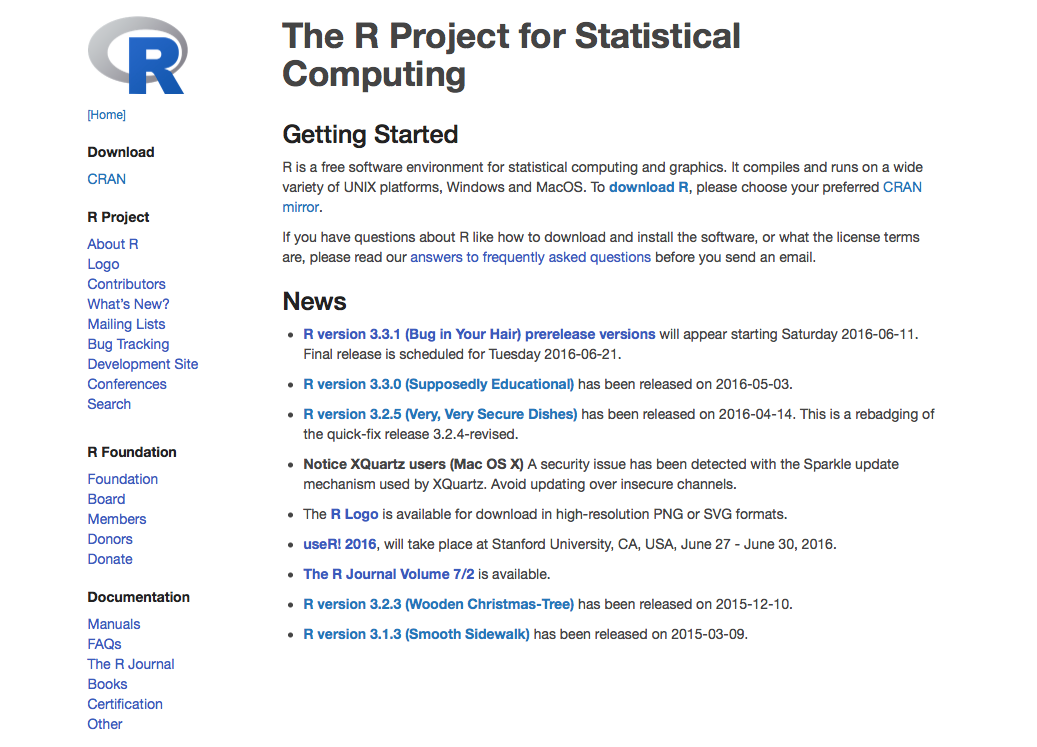
\includegraphics[scale=0.25]{figures/R-project.png} \end{center}
\end{frame}

%%%%%%% 
\begin{frame}
	\frametitle{What R is?}
        \Large The \texttt{R} Project for Statistical Computing\\
	\begin{itemize}
		\small
		\item R version 3.3.1 (released 2016-06-21)
		\item Currently, the CRAN {\tiny(Comprehensive R Archive Network)} package repository features 8609 available packages
			\begin{itemize}
				\item \tiny \url{https://cran.r-project.org/web/packages/available_packages_by_name.html}
			\end{itemize}
		\item Currently, the Bioconductor repository features 1211 available packages
			\begin{itemize}
				\item \tiny \url{http://www.bioconductor.org}
			\end{itemize}
		\item Executed using command line, or a graphical user interface (GUI)
		\item On this course, we use the RStudio GUI
			\begin{itemize}
				\item \tiny \url{www.rstudio.com}
			\end{itemize}
	\end{itemize}
\end{frame}

%%%%%%% 
\begin{frame}[fragile]
	\frametitle{Getting started}
        \begin{itemize}
          \item \texttt{R} is a program which, once installed on your system, can be launched and is immediately ready to take input directly from the user\\
         
  \texttt{R} can be launched in 2 ways:
	  \begin{enumerate}
	    \item From command line
	      \begin{itemize}
		\item To start \texttt{R} you need to enter the console (also called terminal or shell)
		\item To start \texttt{R}, at the prompt simply type: \Large \texttt{R}
	      \end{itemize}
	    \item Using RStudio
	      \begin{itemize}
		  \item To launch RStudio, find the RStudio icon and double-click
		\end{itemize}
	    \end{enumerate}
  \end{itemize}
\end{frame}

%%%%%%% 
\begin{frame}
	\frametitle{RStudio presentation}
	Since we will use RStudio in this course, let's have a look of the program\\
	\centering 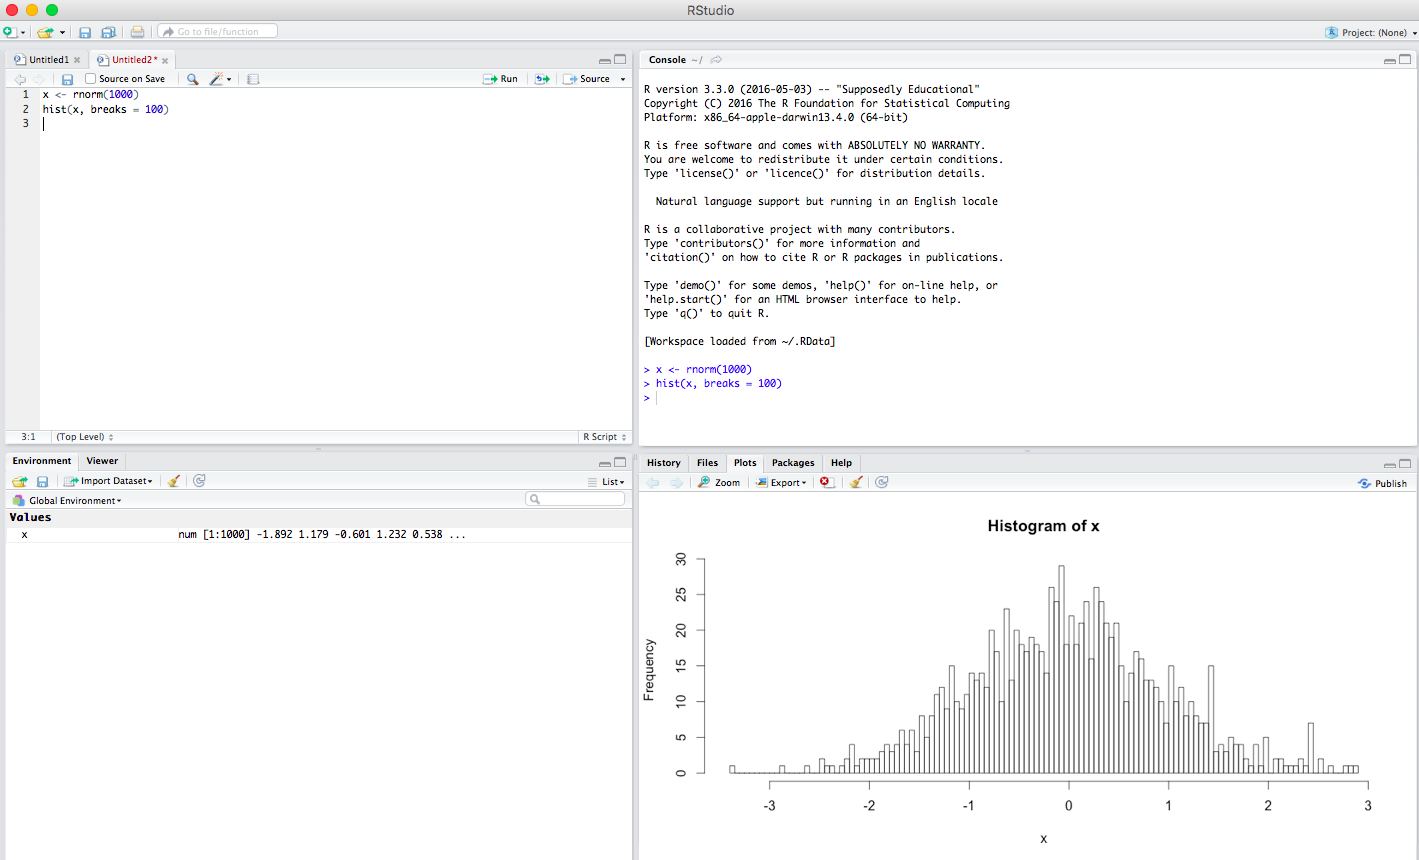
\includegraphics[scale=1.4]{figures/Rstudio_overview.png}
\end{frame}

%%%%%%% 
\begin{frame}
	\frametitle{RStudio presentation}
	\textbf{R console}\\
	\vspace{20pt}
	\centering 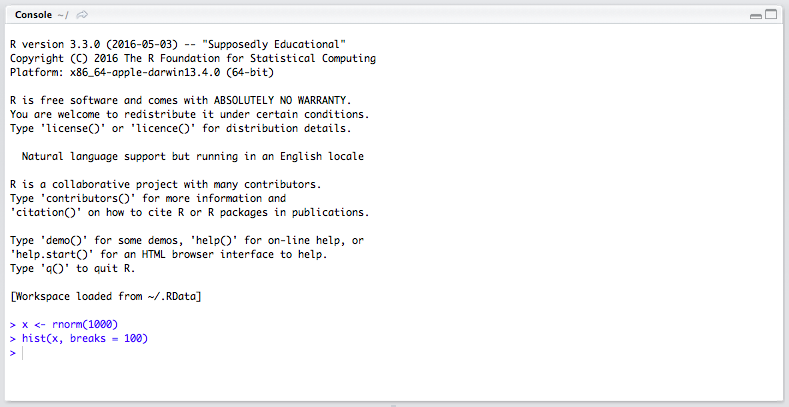
\includegraphics[width=11cm]{figures/RStudio_console.png}\\
	\small It is the place where you can interactively run R commands
\end{frame}

%%%%%%% 
\begin{frame}
	\frametitle{RStudio presentation}
	\textbf{Source editor for R scripts}\\
	\vspace{20pt}
	\centering 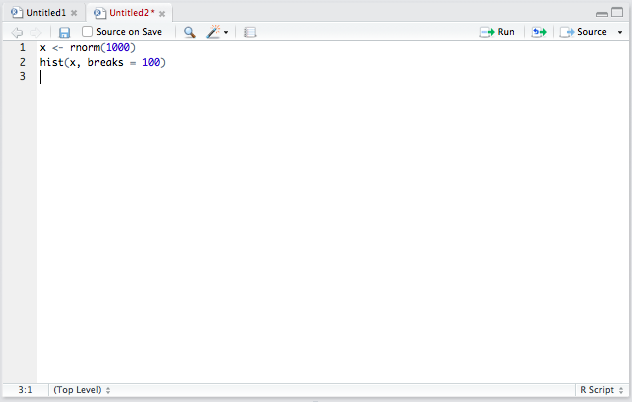
\includegraphics[width=10cm]{figures/RStudio_script.png}\\
	\small It is the place where you can write your scripts
\end{frame}

%%%%%%% 
\begin{frame}
	\frametitle{RStudio presentation}
	\textbf{Workspace}\\
	\vspace{16pt}
	\centering 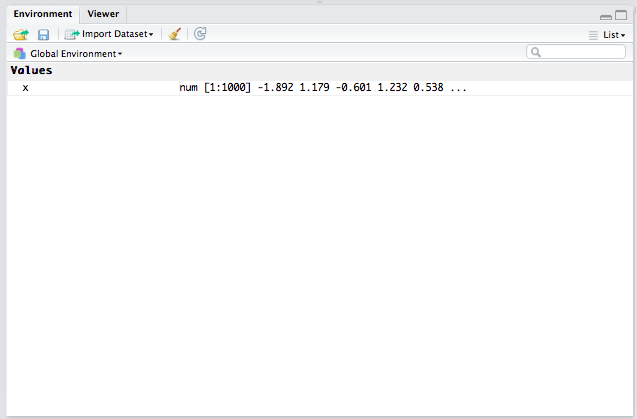
\includegraphics[width=10cm]{figures/RStudio_environment.png}\\
	\small It is the place where you can view object in the global environment
\end{frame}

%%%%%%% 
\begin{frame}
	\frametitle{RStudio presentation}
	\textbf{Plot pannel}\\
	\vspace{20pt}
	\centering 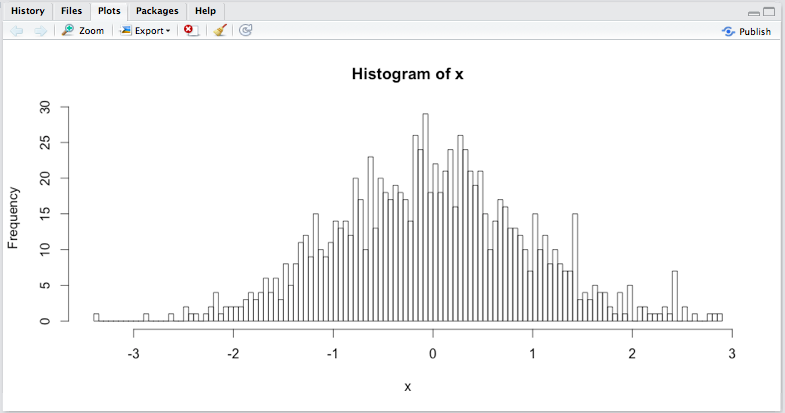
\includegraphics[width=10cm]{figures/RStudio_plot.png}\\
	\small It is the place where you can view your plots
\end{frame}

%%%%%%% 
\begin{frame}
	\frametitle{RStudio presentation}
	\textbf{R help}\\
	\vspace{20pt}
	\centering 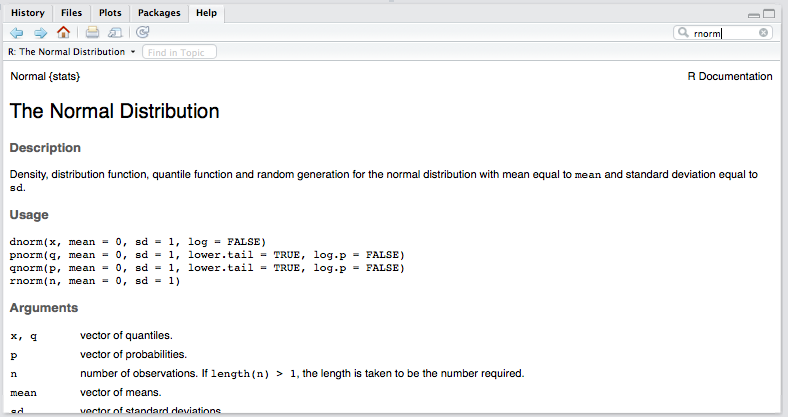
\includegraphics[width=10cm]{figures/RStudio_help.png}\\
	\small It is the place where you can find help
\end{frame}

%%%%%%% 
\begin{frame}
	\frametitle{RStudio presentation}
	The GUI is divided into 4 main sub-windows\\
	These sub-windows are customizable\\
	\vspace{10pt}
	\centering 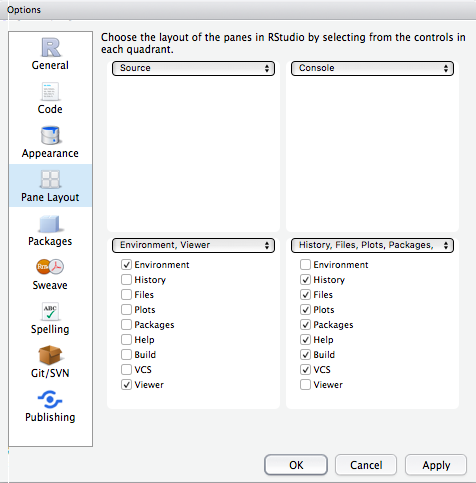
\includegraphics[width=7cm]{figures/RStudio_option.png}
\end{frame}

%%%%%%%%%%%%%%%%%%%%%%%%%%%%%%%%%%%%%%%%%%%%%%%%%%%%%%%%%%%%%%%%%%%%%%
%%%%%%%%%%%%%%%%%%%%%%%%%%%%%%%%%%%%%%%%%%%%%%%%%%%%%%%%%%%%%%%%%%%%%%
\begin{frame}
\section{Basic concepts in R}
\vspace{30pt}
\scriptsize
\begin{flushright}  Based on \url{https://github.com/lgatto/TeachingMaterial/tree/master/\_basicr} \end{flushright}
\end{frame}

%%%%%%% 
\begin{frame}[fragile]{prova}
	\frametitle{The R syntax}
	\begin{center} 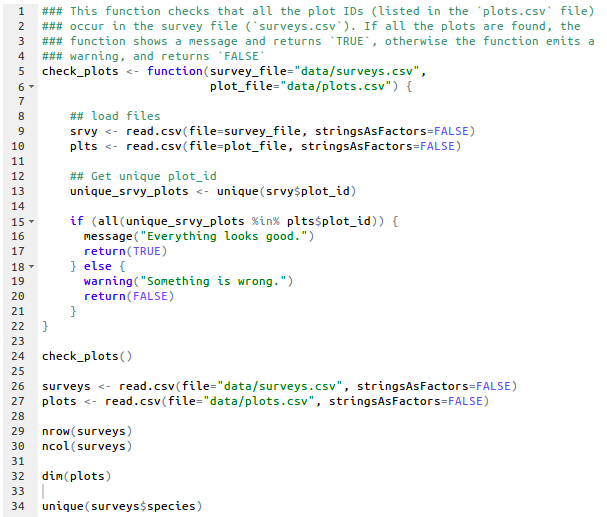
\includegraphics[scale=0.25]{figures/R_syntax.png} \end{center}
\end{frame}

%%%%%%% 
\begin{frame}[fragile]{prova}
	\frametitle{Numbers}
	Element to notice:
	\begin{itemize}
		\item functions
		\item the assignment operator <-
		\item the = for arguments
		\item the comments \# and how they are used to document function and its content
		\item the \$ operator
		\item Point to indentation and consistency in spacing to improve clarity
	\end{itemize}
\end{frame}

%%%%%%% 
\begin{frame}[fragile]{prova}
	\frametitle{Numbers}
	The command line can be used as a calculator
\rule{\textwidth}{0.4pt}
\begin{Schunk}
\begin{Sinput}
> 5 + 7 
\end{Sinput}
\begin{Soutput}
[1] 12
\end{Soutput}
\begin{Sinput}
> 5 - 7
\end{Sinput}
\begin{Soutput}
[1] -2
\end{Soutput}
\begin{Sinput}
> 5 * 7
\end{Sinput}
\begin{Soutput}
[1] 35
\end{Soutput}
\begin{Sinput}
> 5 / 7
\end{Sinput}
\begin{Soutput}
[1] 0.7142857
\end{Soutput}
\end{Schunk}
\rule{\textwidth}{0.4pt}
\vspace{5pt}
\small Note: The number in the square brackets is an indicator of the position in the output
\end{frame}

%%%%%%% 
\begin{frame}[fragile]{prova}
	\frametitle{Numbers}
	You can solve simple or complex calculations 
	\rule{\textwidth}{0.4pt}
\begin{Schunk}
\begin{Sinput}
> (((20/5)^2)-((5+1/3+4/5-10)*(2-34))-20)
\end{Sinput}
\begin{Soutput}
[1] -127.7333
\end{Soutput}
\end{Schunk}
\rule{\textwidth}{0.4pt}
\vspace{20pt}
\Large But, of course, \texttt{R} is not a calculator
\end{frame}

%%%%%%% 
\begin{frame}[fragile]
	\frametitle{Variables}
	A \textbf{variable} is a letter or word which takes (or contains) a value. We use the assignment 'operator', <-\\
	\vspace{10pt}
	- We can assign a number to a variable
	\rule{\textwidth}{0.4pt}
\begin{Schunk}
\begin{Sinput}
> x <- 5
> x
\end{Sinput}
\begin{Soutput}
[1] 5
\end{Soutput}
\end{Schunk}
 \rule{\textwidth}{0.4pt}
 - We can assign the result of an operation to a variable
 \rule{\textwidth}{0.4pt}
\begin{Schunk}
\begin{Sinput}
> y <- 5 + 7
> y
\end{Sinput}
\begin{Soutput}
[1] 12
\end{Soutput}
\end{Schunk}
\rule{\textwidth}{0.4pt}
\end{frame}

%%%%%%% 
\begin{frame}[fragile]
	\frametitle{Variables}
	- We can assign use the variables to perform calculation
	\rule{\textwidth}{0.4pt}
\begin{Schunk}
\begin{Sinput}
> x + y
\end{Sinput}
\begin{Soutput}
[1] 17
\end{Soutput}
\end{Schunk}
 \rule{\textwidth}{0.4pt}
 - We can assign the change the content of the variable
 \rule{\textwidth}{0.4pt}
\begin{Schunk}
\begin{Sinput}
> x
\end{Sinput}
\begin{Soutput}
[1] 5
\end{Soutput}
\begin{Sinput}
> x <- x - y
> x
\end{Sinput}
\begin{Soutput}
[1] -7
\end{Soutput}
\end{Schunk}
\rule{\textwidth}{0.4pt}
\end{frame}

%%%%%%% 
\begin{frame}[fragile]
	\frametitle{Function}
	\textbf{Functions} in \texttt{R} perform operations on arguments (the input(s) to the function). \\ Arguments are always contained in parentheses, i.e. curved brackets (), separated by commas.
	\vspace{10pt}
	
\begin{Schunk}
\begin{Sinput}
> sum(3, 4, 5, 6)
\end{Sinput}
\begin{Soutput}
[1] 18
\end{Soutput}
\begin{Sinput}
> max(3, 4, 5, 6)
\end{Sinput}
\begin{Soutput}
[1] 6
\end{Soutput}
\begin{Sinput}
> min(3, 4, 5, 6)
\end{Sinput}
\begin{Soutput}
[1] 3
\end{Soutput}
\end{Schunk}

\end{frame}

%%%%%%% 
\begin{frame}[fragile]
	\frametitle{Function extention}
	\texttt{R} contains a lot of pre-builtin functions, but through the so called \textit{packages} is possible extend the \texttt{R} functionalities enormously.
	\vspace{30pt}
	Alternatevely, you can write your own function
\begin{Schunk}
\begin{Sinput}
> summ <- function(a,b){ a + b }
> summ(1,2)
\end{Sinput}
\begin{Soutput}
[1] 3
\end{Soutput}
\end{Schunk}
\end{frame}



\subsection{Vector}
%%%%%%% 
\begin{frame}
	\centering \Huge Vector
\end{frame}

%%%%%%% 
\begin{frame}[fragile]
	\frametitle{Vector}
	The basic data structure in \texttt{R} is a \textbf{vector}, an ordered collection of values. \texttt{R} even treats single values as 1-element vectors.\\
	The simplest way to create a \textbf{vector} in \texttt{R} is by using the c() operator:
	\rule{\textwidth}{0.4pt}
\begin{Schunk}
\begin{Sinput}
> c(1,2,3,50)
\end{Sinput}
\begin{Soutput}
[1]  1  2  3 50
\end{Soutput}
\end{Schunk}
\rule{\textwidth}{0.4pt}
\vspace{20pt}
\end{frame}

%%%%%%% 
\begin{frame}[fragile]
	\frametitle{Vector}
	The simplest way to create a \textbf{sequence of numbers} is by using the `:` operator:
	\rule{\textwidth}{0.4pt}
\begin{Schunk}
\begin{Sinput}
> 1:10
\end{Sinput}
\begin{Soutput}
 [1]  1  2  3  4  5  6  7  8  9 10
\end{Soutput}
\end{Schunk}
\rule{\textwidth}{0.4pt}
\vspace{20pt}
That gave us every integer between (and including) 1 and 10.
\end{frame}

%%%%%%% 
\begin{frame}[fragile]
	\frametitle{Vector}
	What happens if we do 15:1? Give it a try to find out.
	\pause
	\rule{\textwidth}{0.4pt}
\begin{Schunk}
\begin{Sinput}
> 15:1
\end{Sinput}
\begin{Soutput}
 [1] 15 14 13 12 11 10  9  8  7  6  5  4  3  2  1
\end{Soutput}
\end{Schunk}
\rule{\textwidth}{0.4pt}\\
\vspace{20pt}
It counted backwards in increments of 1!
\end{frame}

%%%%%%% 
\begin{frame}[fragile]
	\frametitle{Vector}
  	Remember that if you have questions about a particular R function, you can access its documentation with a question mark followed by the function name:\\
\begin{equation}?function name here \end{equation}\\
  However, in the case of an operator like the colon used above, you must enclose the symbol in backticks like this:\\
  \begin{equation}?`: \end{equation}\\
\end{frame}

%%%%%%% 
\begin{frame}[fragile]
	\frametitle{Vector}
	Often, we'll desire more control over a sequence we're creating than what the `:` operator gives us. The seq() function serves this purpose.\\
	\centering Try it: \small Remember what we said about the function arguments\\
	\pause
	\rule{\textwidth}{0.4pt}
\begin{Schunk}
\begin{Sinput}
> seq(1,10)
\end{Sinput}
\begin{Soutput}
 [1]  1  2  3  4  5  6  7  8  9 10
\end{Soutput}
\end{Schunk}
	\rule{\textwidth}{0.4pt}
\end{frame}

%%%%%%% 
\begin{frame}[fragile]
	\frametitle{Vector}
	This gives us the same output as 1:10. However, let's say that instead we want a vector of numbers ranging from 0 to 4, incremented by 0.5. seq(0, 4,by=0.5) does just that.\\
	\centering Try it out.\\
	\pause
	\rule{\textwidth}{0.4pt}
\begin{Schunk}
\begin{Sinput}
> seq(0, 4, by = 0.5)
\end{Sinput}
\begin{Soutput}
[1] 0.0 0.5 1.0 1.5 2.0 2.5 3.0 3.5 4.0
\end{Soutput}
\end{Schunk}
\rule{\textwidth}{0.4pt}
\end{frame}

%%%%%%% 
\begin{frame}[fragile]
	\frametitle{Vector}
	Or maybe we don't care what the increment is and we just want a sequence of 10 numbers between 5 and 10. seq(5, 10, length=10) does the trick. Give it a shot now and store the result in a new variable called \textit{mySeq}.\\
	\centering Try it out.\\
	\pause
\rule{\textwidth}{0.4pt}
\begin{Schunk}
\begin{Sinput}
> mySeq <- seq(5, 10, length=10)
> round(mySeq,1)
\end{Sinput}
\begin{Soutput}
 [1]  5.0  5.6  6.1  6.7  7.2  7.8  8.3  8.9  9.4 10.0
\end{Soutput}
\end{Schunk}
  \rule{\textwidth}{0.4pt}
\end{frame}

%%%%%%% 
\begin{frame}[fragile]
\frametitle{Vector}
To confirm that mySeq has length 10, we can use the length() function.\\
\centering Try it now\\
\pause
\rule{\textwidth}{0.4pt}
\begin{Schunk}
\begin{Sinput}
> length(mySeq)
\end{Sinput}
\begin{Soutput}
[1] 10
\end{Soutput}
\end{Schunk}
  \rule{\textwidth}{0.4pt}
\end{frame}

%%%%%%% 
\begin{frame}[fragile]
	\frametitle{Vector}
	\begin{itemize}
  	\item Let's pretend we don't know the length of mySeq, but we want to generate a sequence of integers from 1 to N, where N represents the length of the mySeq vector.
  	\item We want a new vector (1, 2, 3, ...) that is the same length as mySeq.
  	\item There are several ways we could do this. 
  	\item One possibility is to combine the `:` operator and the length() function.
	\end{itemize}
	\centering Give that a try
	\pause
\rule{\textwidth}{0.4pt}
\begin{Schunk}
\begin{Sinput}
> 1:length(mySeq)
\end{Sinput}
\begin{Soutput}
 [1]  1  2  3  4  5  6  7  8  9 10
\end{Soutput}
\end{Schunk}
\rule{\textwidth}{0.4pt}
\end{frame}

%%%%%%% 
\begin{frame}[fragile]
	\frametitle{Vector}
	Another option is to use seq(along.with = mySeq). Give that a try.
\rule{\textwidth}{0.4pt}
\begin{Schunk}
\begin{Sinput}
> seq(along.with = mySeq)
\end{Sinput}
\begin{Soutput}
 [1]  1  2  3  4  5  6  7  8  9 10
\end{Soutput}
\end{Schunk}
\rule{\textwidth}{0.4pt}\\
\vspace{20pt}
R has a separate built-in function for this purpose
\rule{\textwidth}{0.4pt}
\begin{Schunk}
\begin{Sinput}
> seq_along(mySeq)
\end{Sinput}
\begin{Soutput}
 [1]  1  2  3  4  5  6  7  8  9 10
\end{Soutput}
\end{Schunk}
\rule{\textwidth}{0.4pt}
\end{frame}

%%%%%%% 
\begin{frame}[fragile]
	\frametitle{Vector}
	\begin{itemize}
	\item There are often \textbf{several approaches} to solving the same problem in \texttt{R}          \item Simple approaches that involve \textbf{less typing} are generally best
	\item It is also important for your code to be \textbf{readable}, so that you and others can figure out what's going on without too much hassle
	\end{itemize}
\rule{\textwidth}{0.4pt}
\begin{Schunk}
\begin{Sinput}
> # Create a sequence of 10 numbers
> seq_along(mySeq)
\end{Sinput}
\begin{Soutput}
 [1]  1  2  3  4  5  6  7  8  9 10
\end{Soutput}
\end{Schunk}
\rule{\textwidth}{0.4pt}
\small The comments in \texttt{R} begin with \textbf{hash}. You should have about 1/3 of your code commented. 
\end{frame}

%%%%%%% 
\begin{frame}[fragile]
	\frametitle{Vector}
	One more function related to creating sequences of numbers is rep(), which stands for 'replicate'.\\
	If we're interested in creating a vector that contains 1 and 0 five times, we can use rep(c(1,0), times = 5).\\
	\centering Try it out
	\pause
	\rule{\textwidth}{0.4pt}
\begin{Schunk}
\begin{Sinput}
> # Create a sequence of 1 and 0
> rep(c(1,0), times = 5)
\end{Sinput}
\begin{Soutput}
 [1] 1 0 1 0 1 0 1 0 1 0
\end{Soutput}
\end{Schunk}
\rule{\textwidth}{0.4pt}
\end{frame}

%%%%%%% 
\begin{frame}[fragile]
	\frametitle{Vector}
If we want our vector to contain 5 ones and then 5 zeros, we can do this with the `each` argument instead of `times` argument.\\
  \centering Try it out\\
  \pause
  \rule{\textwidth}{0.4pt}
\begin{Schunk}
\begin{Sinput}
> # Create a sequence of 1 and 0
> rep(c(1,0), each = 5)
\end{Sinput}
\begin{Soutput}
 [1] 1 1 1 1 1 0 0 0 0 0
\end{Soutput}
\end{Schunk}
\rule{\textwidth}{0.4pt}
\end{frame}

%%%%%%% 
\begin{frame}[fragile]
	\frametitle{Vector}
	\begin{itemize}
	\item We'll see, now, how to \textbf{extract} elements from a vector (subset)
	\item The square brackets \textbf{[]} indicate position within the vector
	  \begin{itemize}
	    \small
	    \item \texttt{R} even treats single values as 1-element vectors
	    \item The vector in \texttt{R} starts from position 1
	  \end{itemize}
	\item We can extract individual elements by using the \textbf{[]} notation
  \end{itemize}
  \centering Try mySeq[1:3]\\
  \pause
  \rule{\textwidth}{0.4pt}
\begin{Schunk}
\begin{Sinput}
> mySeq[1:3]
\end{Sinput}
\begin{Soutput}
[1] 5.000000 5.555556 6.111111
\end{Soutput}
\end{Schunk}
\rule{\textwidth}{0.4pt}
\end{frame}

%%%%%%% 
\begin{frame}[fragile]
	\frametitle{Vector}
	If we want to 3th, 5th and 10th elements of the vector mySeq.\\
	\centering Try it out
	\pause
	\rule{\textwidth}{0.4pt}
\begin{Schunk}
\begin{Sinput}
> round(mySeq,1)
\end{Sinput}
\begin{Soutput}
 [1]  5.0  5.6  6.1  6.7  7.2  7.8  8.3  8.9  9.4 10.0
\end{Soutput}
\begin{Sinput}
> round(mySeq[c(3,5,10)],1)
\end{Sinput}
\begin{Soutput}
[1]  6.1  7.2 10.0
\end{Soutput}
\end{Schunk}
  \rule{\textwidth}{0.4pt}
\end{frame}

%%%%%%% 
\begin{frame}[fragile]
	\frametitle{Vector}
	If we want all the elements bigger than 7.\\
	\centering Try it out\\
	\pause
		\rule{\textwidth}{0.4pt}
\begin{Schunk}
\begin{Sinput}
> round(mySeq,1)
\end{Sinput}
\begin{Soutput}
 [1]  5.0  5.6  6.1  6.7  7.2  7.8  8.3  8.9  9.4 10.0
\end{Soutput}
\begin{Sinput}
> round(mySeq[mySeq > 7],1)
\end{Sinput}
\begin{Soutput}
[1]  7.2  7.8  8.3  8.9  9.4 10.0
\end{Soutput}
\end{Schunk}
  \rule{\textwidth}{0.4pt}
\end{frame}

%%%%%%% 
\begin{frame}[fragile]
	\frametitle{Vector}
	If we ask you to produce a vector of 1000 even numbers (from 2 to 2000), extract the 345th and the 987th elements and sum them, would you know how to do it?\\
	\centering Try it out
	\pause
		\rule{\textwidth}{0.4pt}
\begin{Schunk}
\begin{Sinput}
> a <- seq(2,2000,by=2)
> length(a)
\end{Sinput}
\begin{Soutput}
[1] 1000
\end{Soutput}
\begin{Sinput}
> a[345] + a[987]
\end{Sinput}
\begin{Soutput}
[1] 2664
\end{Soutput}
\begin{Sinput}
> # Short version
> sum(seq(2,2000,by=2)[c(345,987)])
\end{Sinput}
\begin{Soutput}
[1] 2664
\end{Soutput}
\end{Schunk}
  \rule{\textwidth}{0.4pt}
\end{frame}

%%%%%%% 
\begin{frame}[fragile]
	\frametitle{Vector}
	When applying all standard arithmetic operations to vectors, \textbf{application is element-wise}.\\
\rule{\textwidth}{0.4pt}
\begin{Schunk}
\begin{Sinput}
> x <- 1:10
> y <- x * 2
> y
\end{Sinput}
\begin{Soutput}
 [1]  2  4  6  8 10 12 14 16 18 20
\end{Soutput}
\end{Schunk}
  \rule{\textwidth}{0.4pt}
\end{frame}


%%%%%%% 
\begin{frame}[fragile]
	\frametitle{Vector}
	Adding two vectors\\
\rule{\textwidth}{0.4pt}
\begin{Schunk}
\begin{Sinput}
> z <- x^2
> y + z
\end{Sinput}
\begin{Soutput}
 [1]   3   8  15  24  35  48  63  80  99 120
\end{Soutput}
\end{Schunk}
  \rule{\textwidth}{0.4pt}\\
  \vspace{20pt}
  If vectors are not the same length, the shorter one will be recycled\\
  \rule{\textwidth}{0.4pt}
\begin{Schunk}
\begin{Sinput}
> x
\end{Sinput}
\begin{Soutput}
 [1]  1  2  3  4  5  6  7  8  9 10
\end{Soutput}
\begin{Sinput}
> x + 1:2
\end{Sinput}
\begin{Soutput}
 [1]  2  4  4  6  6  8  8 10 10 12
\end{Soutput}
\end{Schunk}
  \rule{\textwidth}{0.4pt}
\end{frame}

%%%%%%% 
\begin{frame}[fragile]
	\frametitle{Vector}
	\begin{itemize}
	  \item All the vectors we have seen so far have contained numbers, but we can also store strings 
\rule{\textwidth}{0.4pt}
\footnotesize
\begin{Schunk}
\begin{Sinput}
> gene.names <- c("Pax6","Beta-actin","FoxP2","Hox9")
> gene.names
\end{Sinput}
\begin{Soutput}
[1] "Pax6"       "Beta-actin" "FoxP2"      "Hox9"      
\end{Soutput}
\end{Schunk}
  \rule{\textwidth}{0.4pt}\\
  \vspace{20pt}
  \normalsize
	  \item We can name elements of vectors using the \textit{names} function
\rule{\textwidth}{0.4pt}
\footnotesize
\begin{Schunk}
\begin{Sinput}
> gene.expression <- c(0,3.2,1.2,-2)
> gene.expression
\end{Sinput}
\begin{Soutput}
[1]  0.0  3.2  1.2 -2.0
\end{Soutput}
\begin{Sinput}
> names(gene.expression)<-gene.names
> gene.expression
\end{Sinput}
\begin{Soutput}
      Pax6 Beta-actin      FoxP2       Hox9 
       0.0        3.2        1.2       -2.0 
\end{Soutput}
\end{Schunk}
  \rule{\textwidth}{0.4pt}\\
  \normalsize
	\end{itemize}
	
\end{frame}

%%%%%%% 
\begin{frame}[fragile]
	\frametitle{Vector}
	\Large Exercise: genes and genomes
	\begin{itemize}
	\small
	  \item Let's try some \textbf{vector arithmetic}. Here are the genome lengths and number of protein coding genes for several model organisms:
	  \begin{table}[]
	  \scriptsize
\centering
\begin{tabular}{|l|c|c|}
\hline
\multicolumn{1}{|c|}{Species}     & Genome size (Mb) & Protein coding genes \\ \hline
\textit{Homo sapiens}             & 3,102            & 20,774               \\ \hline
\textit{Mus musculus}             & 2,731            & 23,139               \\ \hline
\textit{Drosophila melanogaster}  & 169              & 13,937               \\ \hline
\textit{Caenorhabditis elegans}   & 100              & 20,532               \\ \hline
\textit{Saccharomyces cerevisiae} & 12               & 6,692                \\ \hline
\end{tabular}
\end{table}
  \item Create \textbf{genome.size} and \textbf{coding.genes} vectors to hold the data in each column using the c function
  \item Create a \textbf{species.name} vector and use this vector to name the values in the other two vectors.
	\end{itemize}
\end{frame}

%%%%%%% 
\begin{frame}[fragile]
	\frametitle{Vector}
	\Large Exercise: genes and genomes
	\begin{itemize}
	\small
	  \item Let's assume a \textbf{coding gene has an average length of 1.5 kilobases} \footnotesize (1.5 kilobases is 0.0015 Megabases)
	  \small
	  \item On average, how many base pairs of each genome is made of coding genes? 
	  \item \textbf{Create a new vector to record this} called \textbf{coding.bases}
	  \item \textbf{What percentage of each genome is made up of protein coding genes?} 
	  \item Use your \textbf{coding.bases} and \textbf{genome.size} vectors to calculate this
	  \item \textbf{How many times more bases are used for coding in the human genome compared to the yeast genome?
	  \item How many times more bases are in the human genome in total compared to the yeast genome?}
	  \item Look up indices of your vectors to find out.
	 \end{itemize}
\end{frame}

%%%%%%% 
\begin{frame}[fragile]
	\frametitle{Vector}
	\Large Exercise: genes and genomes
	\begin{itemize}
	\small
	  \item Creating vectors:
\rule{\textwidth}{0.4pt}
\footnotesize
\begin{Schunk}
\begin{Sinput}
> genome.size<-c(3102,2731,169,100,12)
> coding.genes<-c(20774,23139,13937,20532,6692)
> species.name<-c("H. sapiens","M. musculus","D. melanogaster","C. elegans","S.
+ cerevisiae")
> names(genome.size)<-species.name
> names(coding.genes)<-species.name
\end{Sinput}
\end{Schunk}
  \rule{\textwidth}{0.4pt}\\
  \small
  \pause
    \item To calculate the number of coding bases, we need to use the same scale as we used for genome size: 1.5 kilobases is 0.0015 Megabases
\rule{\textwidth}{0.4pt}
\footnotesize
\begin{Schunk}
\begin{Sinput}
> coding.bases<-coding.genes*0.0015
> coding.bases
\end{Sinput}
\begin{Soutput}
     H. sapiens     M. musculus D. melanogaster      C. elegans  S.\ncerevisiae 
        31.1610         34.7085         20.9055         30.7980         10.0380 
\end{Soutput}
\end{Schunk}
  \rule{\textwidth}{0.4pt}\\
	\end{itemize}
\end{frame}

%%%%%%% 
\begin{frame}[fragile]
	\frametitle{Vector}
	\Large Exercise: genes and genomes
	\begin{itemize}
	\small
	  \item To calculate the percentage of coding bases in each genome:
\rule{\textwidth}{0.4pt}
\footnotesize
\begin{Schunk}
\begin{Sinput}
> coding.pc<-coding.bases/genome.size*100
> coding.pc
\end{Sinput}
\begin{Soutput}
     H. sapiens     M. musculus D. melanogaster      C. elegans  S.\ncerevisiae 
       1.004545        1.270908       12.370118       30.798000       83.650000 
\end{Soutput}
\end{Schunk}
  \rule{\textwidth}{0.4pt}\\
  \small
  \pause
    \item To compare human to yeast:
\rule{\textwidth}{0.4pt}
\footnotesize
\begin{Schunk}
\begin{Sinput}
> coding.bases[1]/coding.bases[5]
\end{Sinput}
\begin{Soutput}
H. sapiens 
  3.104304 
\end{Soutput}
\begin{Sinput}
> genome.size[1]/genome.size[5]
\end{Sinput}
\begin{Soutput}
H. sapiens 
     258.5 
\end{Soutput}
\end{Schunk}
  \rule{\textwidth}{0.4pt}\\
	\end{itemize}
\end{frame}

%%%%%%% 
\begin{frame}[fragile]
	\frametitle{Vector}
	\Large Exercise: genes and genomes
	\begin{itemize}
	\small
	  \item Note that if a new vector is created using a named vector, the names are usually carried across to the new vector. Sometimes this is what we want (as for \textbf{coding.pc}) but sometimes it is not (when we are comparing human to yeast). We can remove names by setting them to the special NULL value:
\rule{\textwidth}{0.4pt}
\footnotesize
\begin{Schunk}
\begin{Sinput}
> names(coding.pc)<-NULL
> coding.pc
\end{Sinput}
\begin{Soutput}
[1]  1.004545  1.270908 12.370118 30.798000 83.650000
\end{Soutput}
\end{Schunk}
  \rule{\textwidth}{0.4pt}\\
	\end{itemize}
\end{frame}

\subsection{R packages}
\begin{frame}
	\centering \Huge R packages
\end{frame}

\begin{frame}[fragile]
	\frametitle{R packages}
	\begin{itemize}
	\small
\item \texttt{R} comes ready loaded with various libraries of functions called \textbf{packages}. e.g. the function \textbf{sum()} is in the base package and \textbf{sd()}, which calculates the standard deviation of a vector, is in the stats package
	\pause
		\item There are 1000s of additional packages provided by third parties, and the packages can be found in numerous server locations on the web called repositories
	\pause
		\item The two repositories you will come across the most are
			\begin{itemize}
				\item The Comprehensive R Archive Network (CRAN)
				\item Bioconductor
			\end{itemize}
	\pause
		\item CRAN is mirrored in many locations. Set your local mirror in RStudio using Tools > Options, and choose a CRAN mirror
	\pause
		\item Bioconductor packages are then loaded with the biocLite() function
			\begin{itemize}
				\item source(``http://bioconductor.org/biocLite.R'')
				\item biocLite(``PackageName'')
			\end{itemize}
	\end{itemize}
\end{frame}

 
\begin{frame}[fragile]
	\frametitle{R package}
	\centering \Huge Exercise
	\begin{itemize}
	\small
		\item Matrix is a CRAN extras package
			\begin{itemize}
				\item Use \textbf{install.packages()} function\ldots
			%	\item install.packages(``Matrix'')
				\item or in RStudio go to Tools > Install Packages\ldots and type the package name
			\end{itemize}
		\item aCGH is a BioConductor package (www.bioconductor.org)
		%	\begin{itemize}
			%	\item source(``http://bioconductor.org/biocLite.R'') 
			%	\item biocLite(``aCGH'')
		%	\end{itemize}
	\end{itemize}
\end{frame}

\begin{frame}[fragile]
	\frametitle{R package}
	\begin{itemize}
	\small
		\item \texttt{R} needs to be told to use the new functions from the installed packages 
		\item Use \textbf{library(\ldots)} function to load the newly installed features
		\item \textbf{library(``Matrix'')};  loads matrix functions
	\end{itemize}
	\footnotesize PS: library(): Lists all the packages you've got installed locally\\
	PS2: .libPaths(): to know where the libraries are installed
\end{frame}


\subsection{Data structures}
%%%%%%
\begin{frame}
	\centering \Large {\sc DATA STRUCTURES}
\end{frame}


%%%%%%% 
\begin{frame}[fragile]
	\frametitle{Data structures}
	\centering \LARGE \texttt{R} is designed to handle experimental data
	\begin{itemize}
		\small
		\item In this lesson, we'll cover \textbf{matrices} and \textbf{data frames}. Both represent 'rectangular' data types, meaning that they are used to store tabular data, with rows and columns
		\item The main difference, as you'll see, is that \textbf{matrices} can only contain a single class of data, while \textbf{data frames} can consist of many different classes of data
	\end{itemize}
\end{frame}

%%%%%%% 
\begin{frame}[fragile]
	\frametitle{Data frame}
	\begin{itemize}
		\small
		\item A data frame is a \textbf{set of observations} of a set of variables  in other words, the \underline{outcome of an experiment}.\\ 
			\tiny [Wickham, H. (2014). Tidy Data. Journal of Statistical Software, 59(10), 1 - 23] 
\pause
	\small
	\item Tidy datasets provide a standardized way to link the structure of a dataset (\textbf{its physical layout}) with its semantics (\textbf{its meaning})	
	\end{itemize}
	\begin{center} 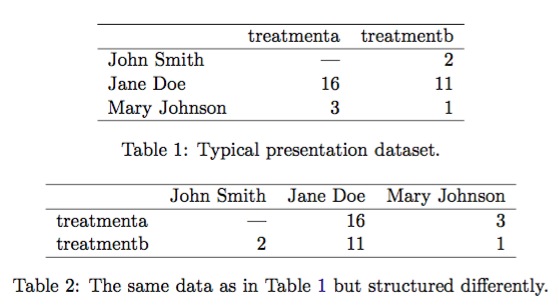
\includegraphics[scale=0.25]{figures/hw_tidy1.png} \end{center}
 
\end{frame}

%%%%%%% 
\begin{frame}[fragile]
	\frametitle{Data frame}
	\begin{itemize}
		\small
		\item A dataset is a collection of \textbf{values}
			\pause
		\item Every value belongs to a \textbf{variable} and an \textbf{observation}
			\pause
		\item A \underline{variable} contains all values that \textbf{measure the same underlying attribute} (like height, temperature, duration) across units
			\pause
		\item An \underline{observation} contains all values \textbf{measured on the same unit} (like a person, or a day, or a race) across attributes
	\end{itemize}
	\begin{center} 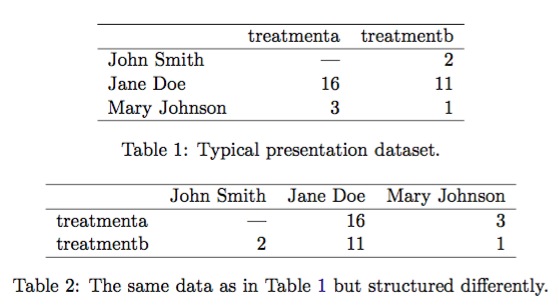
\includegraphics[scale=0.25]{figures/hw_tidy1.png} \end{center}
 
\end{frame}

%%%%%%
\begin{frame}[fragile]
	\frametitle{Data frame}
	\begin{itemize}
		\small
	\item Table 3 reorganizes Table 1 to make the values, variables and observations more clear 
	\item The dataset contains 18 values representing three variables and six observations; the variables are:
		\begin{enumerate}
			\item \textbf{person}, with three possible values (John Smith, Mary Johnson, and Jane Doe)
			\item \textbf{Treatment}, with two possible values (a and b)
			\item \textbf{Result}, with five or six values depending on how you think of the missing value (NA, 16, 3, 2, 11, 1)
		\end{enumerate}
	\end{itemize}
	\begin{center} 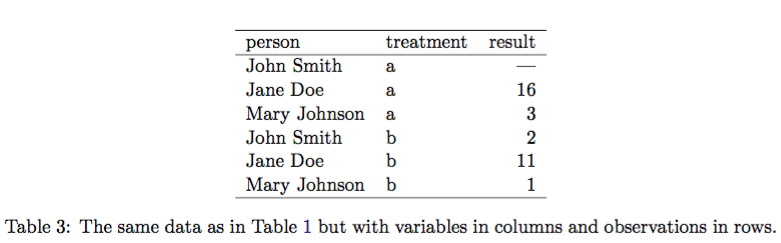
\includegraphics[scale=0.25]{figures/hw_tidy2.png} \end{center}
 
\end{frame}

%%%%%%
\begin{frame}[fragile]
	\frametitle{Data frame}
	\begin{itemize}
		\item A dataset is messy or tidy depending on how rows, columns and tables are matched up with observations, variables and types
		\item In tidy data:
			\begin{enumerate}
		\pause
				\item Each variable forms a column
		\pause
				\item Each observation forms a row
		\pause
				\item Each type of observational unit forms a table
			\end{enumerate}
		\pause
		\item Three common problems with messy datasets are:
	\end{itemize}
\end{frame}
%%%%%%%
%%%%%%
\begin{frame}[fragile]
	\frametitle{Data frame}
	\centering \large \underline{Column headers are values, not variable names}
	\vspace{5pt}

	\begin{center} 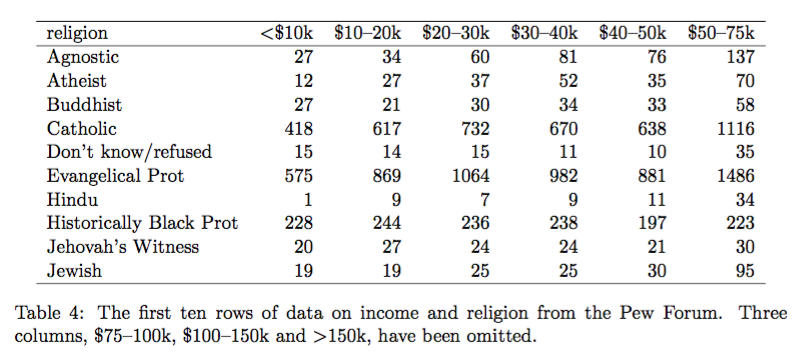
\includegraphics[scale=4.5]{figures/hw_tidy3-1.png} \end{center}
\end{frame} 
%%%%%%
\begin{frame}[fragile]
	\frametitle{Data frame}
	\centering \large \underline{Column headers are values, not variable names}
	\vspace{5pt}

	\begin{center}	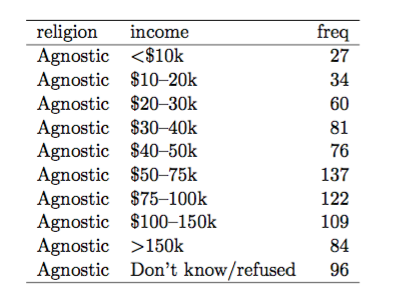
\includegraphics[scale=0.25]{figures/hw_tidy3-2.png} \end{center}
\end{frame} 

%%%%%%
\begin{frame}[fragile]
	\frametitle{Data frame}
	\centering \large \underline{Multiple variables stored in one column}
	\vspace{5pt}

	\begin{center} 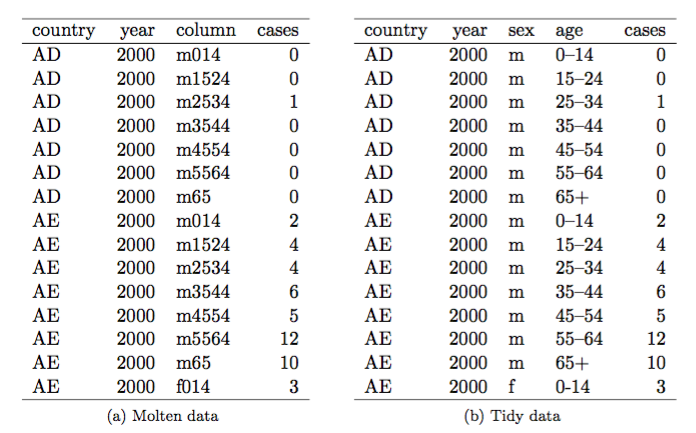
\includegraphics{figures/hw_tidy4.png} \end{center}
\end{frame} 


%%%%%%
\begin{frame}[fragile]
	\frametitle{Data frame}
	\centering \large \underline{Variables are stored in both rows and columns}
	\vspace{5pt}

	\begin{center} 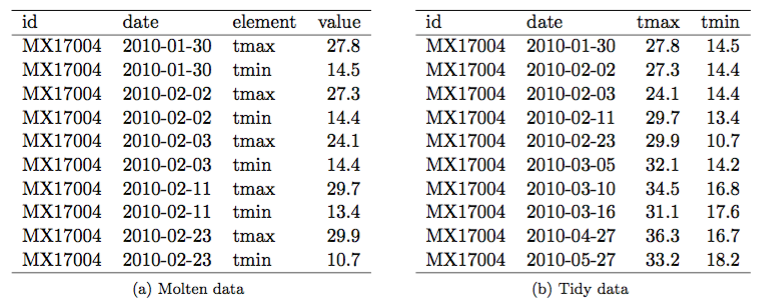
\includegraphics{figures/hw_tidy5.png} \end{center}
\end{frame} 

%%%%%%
\begin{frame}[fragile]
	\frametitle{Data frame}
	\begin{itemize}
		\small
	\item For example, we might want to analyse information about a \underline{set of patients}. To start with, let's say we have ten patients and for each one we know their \textbf{name, sex, age, weight and whether they give consent} for their data to be made public
\pause
		\item We are going to create a data frame called 'patients', which will have \underline{ten rows (observations)} and \underline{seven columns (variables)}. 
		\item \textbf{The columns must all be equal lengths}

	\end{itemize}
\end{frame}

%%%%%%% 

\begin{frame}[fragile]
	\frametitle{Data frame}
	\centering \LARGE The patients data frame
	\vspace{20pt}
\tiny
\begin{Schunk}
\begin{Sinput}
> patients
\end{Sinput}
\begin{Soutput}
   firstName secondName paste.firstName..secondName.    sex age weight consent
1       Adam      Jones                   Adam Jones   Male  50   70.8    TRUE
2        Eve     Parker                   Eve Parker Female  21   67.9    TRUE
3       John      Evans                   John Evans   Male  35   75.3   FALSE
4       Mary      Davis                   Mary Davis Female  45   61.9    TRUE
5      Peter      Baker                  Peter Baker   Male  28   72.4   FALSE
6       Paul    Daniels                 Paul Daniels   Male  31   69.9   FALSE
7     Joanna    Edwards               Joanna Edwards Female  42   63.5   FALSE
8    Matthew      Smith                Matthew Smith   Male  33   71.5    TRUE
9      David    Roberts                David Roberts   Male  57   73.2   FALSE
10     Sally     Wilson                 Sally Wilson Female  62   64.8    TRUE
\end{Soutput}
\end{Schunk}
\small
\end{frame}

%%%%%%% 
\begin{frame}[fragile]
	\frametitle{Data frame}
	\begin{itemize}
		\small
		\item \textbf{Each column is a vector}, like previous vectors we have seen, for example:
\rule{\textwidth}{0.4pt}
\scriptsize
\begin{Schunk}
\begin{Sinput}
> age<-c(50, 21, 35, 45, 28, 31, 42, 33, 57, 62)
> weight<-c(70.8, 67.9, 75.3, 61.9, 72.4, 69.9, 63.5, 71.5, 73.2, 64.8)
\end{Sinput}
\end{Schunk}
\rule{\textwidth}{0.4pt}\\
\small
\vspace{10pt}
\pause
		\item We can define the names using character vectors:
\rule{\textwidth}{0.4pt}
\scriptsize
\begin{Schunk}
\begin{Sinput}
> firstName<-c('Adam', 'Eve', 'John', 'Mary', 'Peter', 'Paul', 
+ 	     'Joanna','Matthew', 'David', 'Sally')
> secondName<-c('Jones', 'Parker', 'Evans', 'Davis', 'Baker', 
+ 	       'Daniels', 'Edwards', 'Smith', 'Roberts', 'Wilson')
\end{Sinput}
\end{Schunk}
\rule{\textwidth}{0.4pt}\\
\small
\vspace{10pt}
\pause
		\item We also have a new type of vector, the logical vector, which only contains the values TRUE and FALSE:
\rule{\textwidth}{0.4pt}
\scriptsize
\begin{Schunk}
\begin{Sinput}
> consent<-c(TRUE,TRUE,FALSE,TRUE,FALSE,FALSE,FALSE,TRUE,FALSE,TRUE)
\end{Sinput}
\end{Schunk}
\rule{\textwidth}{0.4pt}\\\end{itemize}
\end{frame}


%%%%%%% 
\begin{frame}[fragile]
	\frametitle{Data structures}
	\begin{itemize}
		\small
		\item \textbf{Vectors can only contain one type of data}; we cannot mix numbers, characters and logical values in the same vector 
		\item If we try this, \texttt{R} will convert everything to characters:
\rule{\textwidth}{0.4pt}
\scriptsize
\begin{Schunk}
\begin{Sinput}
> c(20, 'a string', TRUE)
\end{Sinput}
\begin{Soutput}
[1] "20"       "a string" "TRUE"    
\end{Soutput}
\end{Schunk}
\rule{\textwidth}{0.4pt}\\
\small
\vspace{10pt}
		\item We can see the type of a particular vector using the mode function
\rule{\textwidth}{0.4pt}
\footnotesize
\setlength{\fancyvrbtopsep}{-1pt}
\setlength{\fancyvrbpartopsep}{-1pt}
\begin{Schunk}
\begin{Sinput}
> mode(firstName)
\end{Sinput}
\begin{Soutput}
[1] "character"
\end{Soutput}
\begin{Sinput}
> mode(age)
\end{Sinput}
\begin{Soutput}
[1] "numeric"
\end{Soutput}
\begin{Sinput}
> mode(weight)
\end{Sinput}
\begin{Soutput}
[1] "numeric"
\end{Soutput}
\begin{Sinput}
> mode(consent)
\end{Sinput}
\begin{Soutput}
[1] "logical"
\end{Soutput}
\end{Schunk}
\rule{\textwidth}{0.4pt}\\
		\small
\vspace{10pt}
	\end{itemize}
\end{frame}


%%%%%%% 
\begin{frame}[fragile]
	\frametitle{Data structures}
	\begin{itemize}
		\small
		\item Character vectors are fine for some variables, like names
		\item But sometimes we have categorical data and we want \texttt{R} to recognize this
		\item \textbf{A factor is \texttt{R}'s data structure for categorical data}
\rule{\textwidth}{0.4pt}
\scriptsize
\setlength{\fancyvrbtopsep}{-1pt}
\setlength{\fancyvrbpartopsep}{-1pt}
\begin{Schunk}
\begin{Sinput}
> sex
\end{Sinput}
\begin{Soutput}
 [1] "Male"   "Female" "Male"   "Female" "Male"   "Male"   "Female" "Male"  
 [9] "Male"   "Female"
\end{Soutput}
\begin{Sinput}
> factor(sex)
\end{Sinput}
\begin{Soutput}
 [1] Male   Female Male   Female Male   Male   Female Male   Male   Female
Levels: Female Male
\end{Soutput}
\end{Schunk}
\rule{\textwidth}{0.4pt}\\
\small
\vspace{10pt}
		\item \texttt{R} has converted the strings of the sex character vector into two levels, which are the categories in the data
		\item Note the values of this factor are not character strings, but \texttt{levels}
		\item We can use this factor to compare data for males and females
	\end{itemize}
\end{frame}


%%%%%%% 
\begin{frame}[fragile]
	\frametitle{Data structures}
	\centering \LARGE Creating a data frame
	\begin{itemize}
		\small
		\item We can construct a data frame from other objects
\rule{\textwidth}{0.4pt}
\tiny
\begin{Schunk}
\begin{Sinput}
> patients<-data.frame(firstName, secondName, paste(firstName,secondName),
+ 		     sex, age, weight, consent)
> patients
\end{Sinput}
\begin{Soutput}
   firstName secondName paste.firstName..secondName.    sex age weight consent
1       Adam      Jones                   Adam Jones   Male  50   70.8    TRUE
2        Eve     Parker                   Eve Parker Female  21   67.9    TRUE
3       John      Evans                   John Evans   Male  35   75.3   FALSE
4       Mary      Davis                   Mary Davis Female  45   61.9    TRUE
5      Peter      Baker                  Peter Baker   Male  28   72.4   FALSE
6       Paul    Daniels                 Paul Daniels   Male  31   69.9   FALSE
7     Joanna    Edwards               Joanna Edwards Female  42   63.5   FALSE
8    Matthew      Smith                Matthew Smith   Male  33   71.5    TRUE
9      David    Roberts                David Roberts   Male  57   73.2   FALSE
10     Sally     Wilson                 Sally Wilson Female  62   64.8    TRUE
\end{Soutput}
\end{Schunk}
\rule{\textwidth}{0.4pt}\\
\small
		\item The paste function joins character vectors together
		\item We can access particular variables using the dollar operator
\rule{\textwidth}{0.4pt}
\tiny
\begin{Schunk}
\begin{Sinput}
> patients$age
\end{Sinput}
\begin{Soutput}
 [1] 50 21 35 45 28 31 42 33 57 62
\end{Soutput}
\end{Schunk}
\rule{\textwidth}{0.4pt}\\
\small
	\end{itemize}
\end{frame}

%%%%%%% 
\begin{frame}[fragile]
	\frametitle{Data structures}
	\centering \LARGE Naming data frame variables
	\begin{itemize}
		\small
		\item \texttt{R} has inferred the names of our data frame variables from the names of the vectors or the commands (eg the paste command)
		\item We can name the variables after we have created a data frame using the \textbf{names} function, and we can use the same function to see the names
\rule{\textwidth}{0.4pt}
\tiny
\begin{Schunk}
\begin{Sinput}
> names(patients)<-c('First_Name', 'Second_Name', 'Full_Name', 'Sex',
+ 		   'Age', 'Weight', 'Consent')
> names(patients)
\end{Sinput}
\begin{Soutput}
[1] "First_Name"  "Second_Name" "Full_Name"   "Sex"         "Age"        
[6] "Weight"      "Consent"    
\end{Soutput}
\end{Schunk}
\rule{\textwidth}{0.4pt}\\
\vspace{10pt}
\small
		\item Or we can name the variables when we define the data frame
\rule{\textwidth}{0.4pt}
\tiny
\begin{Schunk}
\begin{Sinput}
> patients<-data.frame(First_Name=firstName, Second_Name=secondName,
+ 		     Full_Name=paste(firstName,secondName), Sex=sex,
+ 		     Age=age, Weight=weight, Consent=consent)
> names(patients)
\end{Sinput}
\begin{Soutput}
[1] "First_Name"  "Second_Name" "Full_Name"   "Sex"         "Age"        
[6] "Weight"      "Consent"    
\end{Soutput}
\end{Schunk}
\rule{\textwidth}{0.4pt}\\
\small
	\end{itemize}
\end{frame}

%%%%%%% 
\begin{frame}[fragile]
	\frametitle{Data structures}
	\centering \LARGE Matrices
	\begin{itemize}
		\small
	\item Data frames are \texttt{R} speciality, but \texttt{R} also handles matrices
\rule{\textwidth}{0.4pt}
\tiny
\begin{Schunk}
\begin{Sinput}
> e <- matrix(1:10, nrow=5, ncol=2)
> e
\end{Sinput}
\begin{Soutput}
     [,1] [,2]
[1,]    1    6
[2,]    2    7
[3,]    3    8
[4,]    4    9
[5,]    5   10
\end{Soutput}
\end{Schunk}
\vspace{20pt}
\begin{Schunk}
\begin{Sinput}
> f <-  matrix(1:10, nrow=2, ncol=5)
> f
\end{Sinput}
\begin{Soutput}
     [,1] [,2] [,3] [,4] [,5]
[1,]    1    3    5    7    9
[2,]    2    4    6    8   10
\end{Soutput}
\end{Schunk}
\rule{\textwidth}{0.4pt}\\
\small
	\end{itemize}
\end{frame}



%%%%%%% 
\begin{frame}[fragile]
	\frametitle{Data structures}
	\centering \LARGE Lists
	\begin{itemize}
		\small
		\item We have seen that vectors can only hold data of one type. 
		\item \underline{How can we store data of multiple types?} 
		\item \underline{Or vectors of different lengths in one object?}
		\item We can use lists; a list can contain \textbf{objects of any type}
\rule{\textwidth}{0.4pt}
\tiny
\begin{Schunk}
\begin{Sinput}
> a <- 1:10
> b <- matrix(runif(100),ncol=10,nrow=10)
> c <- data.frame(a, month.name[1:10])
> myList<-list( ls.obj.1=a, ls.obj.2=b,ls.obj.3=c )
> summary(myList)
\end{Sinput}
\begin{Soutput}
         Length Class      Mode   
ls.obj.1  10    -none-     numeric
ls.obj.2 100    -none-     numeric
ls.obj.3   2    data.frame list   
\end{Soutput}
\end{Schunk}
\vspace{20pt}
\setlength{\fancyvrbtopsep}{-1pt}
\setlength{\fancyvrbpartopsep}{-1pt}
\begin{Schunk}
\begin{Sinput}
> names(myList)
\end{Sinput}
\begin{Soutput}
[1] "ls.obj.1" "ls.obj.2" "ls.obj.3"
\end{Soutput}
\end{Schunk}

\rule{\textwidth}{0.4pt}\\
\small
	\end{itemize}
\end{frame}


%%%%%%% 
\begin{frame}[fragile]
	\frametitle{Data structures}
	\centering \LARGE Indexing data frames and matrices
	\begin{itemize}
		\small
		\item You can index multidimensional data structures like:\\ \Large \textbf{object [ rows , columns ]}
		\small
		\item If you don't provide an index for either rows or columns, all of the rows or columns will be returned
\rule{\textwidth}{0.4pt}
\tiny
\setlength{\fancyvrbtopsep}{-1pt}
\setlength{\fancyvrbpartopsep}{-1pt}
\begin{Schunk}
\begin{Sinput}
> patients[1,2]
\end{Sinput}
\begin{Soutput}
[1] Jones
10 Levels: Baker Daniels Davis Edwards Evans Jones Parker Roberts ... Wilson
\end{Soutput}
\end{Schunk}
\vspace{20pt}
\setlength{\fancyvrbtopsep}{-1pt}
\setlength{\fancyvrbpartopsep}{-1pt}
\begin{Schunk}
\begin{Sinput}
> patients[1,]
\end{Sinput}
\begin{Soutput}
  First_Name Second_Name  Full_Name  Sex Age Weight Consent
1       Adam       Jones Adam Jones Male  50   70.8    TRUE
\end{Soutput}
\end{Schunk}
\vspace{20pt}
\begin{Schunk}
\begin{Sinput}
> patients[patients$Age>50, ]
\end{Sinput}
\begin{Soutput}
   First_Name Second_Name     Full_Name    Sex Age Weight Consent
9       David     Roberts David Roberts   Male  57   73.2   FALSE
10      Sally      Wilson  Sally Wilson Female  62   64.8    TRUE
\end{Soutput}
\end{Schunk}
\rule{\textwidth}{0.4pt}\\
\small
	\end{itemize}
\end{frame}

%%%%%%% 
\begin{frame}[fragile]
	\frametitle{Data structures}
	\centering \LARGE Indexing data frames and matrices
	\begin{itemize}
		\small
		\item There is a simpler way to refer to variables by name in a \textbf{data frame}
		\item Namely separating the \textbf{data frame name} from the \textbf{name of the variable} with a dollar sign \textbf{(\$)}
\rule{\textwidth}{0.4pt}
\scriptsize
\setlength{\fancyvrbtopsep}{-1pt}
\setlength{\fancyvrbpartopsep}{-1pt}
\begin{Schunk}
\begin{Sinput}
> patients$Age
\end{Sinput}
\begin{Soutput}
 [1] 50 21 35 45 28 31 42 33 57 62
\end{Soutput}
\begin{Sinput}
> patients$Age < 30
\end{Sinput}
\begin{Soutput}
 [1] FALSE  TRUE FALSE FALSE  TRUE FALSE FALSE FALSE FALSE FALSE
\end{Soutput}
\end{Schunk}

\rule{\textwidth}{0.4pt}\\
\small
	\end{itemize}
\end{frame}



%%%%%%% 
\begin{frame}[fragile]
	\frametitle{Data structures}
	\centering \LARGE Advanced indexing
	\begin{itemize}
		\small
		\item As values in R are really vectors, so indices are actually vectors, and can be numeric or logical
\rule{\textwidth}{0.4pt}
\scriptsize
\setlength{\fancyvrbtopsep}{-1pt}
\setlength{\fancyvrbpartopsep}{-1pt}
\begin{Schunk}
\begin{Sinput}
> s <- letters[1:5]
> s
\end{Sinput}
\begin{Soutput}
[1] "a" "b" "c" "d" "e"
\end{Soutput}
\begin{Sinput}
> s[c(TRUE, FALSE, TRUE, FALSE, FALSE)]
\end{Sinput}
\begin{Soutput}
[1] "a" "c"
\end{Soutput}
\begin{Sinput}
> a<-1:5
> a<3
\end{Sinput}
\begin{Soutput}
[1]  TRUE  TRUE FALSE FALSE FALSE
\end{Soutput}
\begin{Sinput}
> s[a<3]
\end{Sinput}
\begin{Soutput}
[1] "a" "b"
\end{Soutput}
\begin{Sinput}
> s[a>1 & a<3]
\end{Sinput}
\begin{Soutput}
[1] "b"
\end{Soutput}
\begin{Sinput}
> s[a==2]
\end{Sinput}
\begin{Soutput}
[1] "b"
\end{Soutput}
\end{Schunk}

\rule{\textwidth}{0.4pt}\\
\small
	\end{itemize}
\end{frame}

%%%%%%% 
\begin{frame}[fragile]
	\frametitle{Data structures}
	\centering \LARGE Operators
	\begin{itemize}
		\small
		\item arithmetic\\ \^{} ,/ ,* ,- , +
		\item comparison\\ =! ,== ,=> ,<= ,> ,<
		\item logical\\ !, \&, |
	\end{itemize}
\end{frame}

%%%%%%% 
\begin{frame}[fragile]
	\frametitle{Data structures}
	\centering \LARGE Exercise
	\begin{itemize}
		\small
		\item Create a data.frame using the following vectors
			\begin{itemize}
				\item n = 1, 2, 3, 4, 5, 6, 7, 8, 9, 10
				\item sex = male, female, male, female, male, female, male, female, male, female 
				\item age = 23, 22, 21, 22, 24, 30, 23, 29, 19, 29
				\item weight = 72, 90, 120, 80, 75, 65, 91, 58, 78, 50
				\item height = 171, 185, 210, 170, 189, 150, 168, 165, 188, 143
			\end{itemize}
	\end{itemize}
\end{frame}

%%%%%%% 
\begin{frame}[fragile]
	\frametitle{Data structures}
	\centering \LARGE Exercise
	\begin{itemize}
		\small
		\item Which is the average age? \tiny [use the function \textbf{mean}]\small
		\item Which is the maximum female weight? \tiny [Subset the data frame and use the function \textbf{max}]\small
		\item Which is the minimum male weight? \tiny [Subset the data frame and use the function \textbf{min}]\small
		\item How many are the male over 180cm? \tiny [Subset the data frame] \small
		\item Which is their average age?
		\item Who is the younger and lighter female? \tiny [this has to be done in 2 steps; use the function \textbf{order}]\small
		\item Who is the person with the minimum BMI \tiny [weight/height\textsuperscript{2}; this also has to be done in 2 steps; use the function \textbf{which.min}]\small
	\end{itemize}
	\small
	\begin{flushleft} 
	\textbf{NOTE}:\\ 
	1. To know how to use a function use '?'; e.g. ?mean\\
	2. In \texttt{R} there are several ways to achieve the same result
	\end{flushleft} 
\end{frame}


%%%%%%% 
\begin{frame}[fragile]
	\frametitle{Data structures}
	\centering \LARGE Exercise
	\begin{itemize}
		\small
		\item Create a data.frame using the following vectors 
\rule{\textwidth}{0.4pt}\\
\tiny
\setlength{\fancyvrbtopsep}{-1pt}
\setlength{\fancyvrbpartopsep}{-1pt}
\begin{Schunk}
\begin{Sinput}
> n <- 1:10
> sex <- rep(c('male', 'female'), 5)
> age <- c(23, 22, 21, 22, 24, 30, 23, 29, 19, 29)
> weight <- c(72, 90, 120, 80, 75, 65, 91, 58, 78, 50)
> height <- c(171, 185, 210, 170, 189, 150, 168, 165, 188, 143)
> df <- data.frame(n = n, sex = sex, age = age, weight = weight, height = height)
> df
\end{Sinput}
\begin{Soutput}
    n    sex age weight height
1   1   male  23     72    171
2   2 female  22     90    185
3   3   male  21    120    210
4   4 female  22     80    170
5   5   male  24     75    189
6   6 female  30     65    150
7   7   male  23     91    168
8   8 female  29     58    165
9   9   male  19     78    188
10 10 female  29     50    143
\end{Soutput}
\end{Schunk}

\rule{\textwidth}{0.4pt}\\
\small
	\end{itemize}
\end{frame}


%%%%%%% 
\begin{frame}[fragile]
	\frametitle{Data structures}
	\centering \LARGE Exercise
	\begin{itemize}
		\small
		\item Which is the average age?
\pause
\rule{\textwidth}{0.4pt}\\
\tiny
\setlength{\fancyvrbtopsep}{-1pt}
\setlength{\fancyvrbpartopsep}{-1pt}
\begin{Schunk}
\begin{Sinput}
> mean(df$age)
\end{Sinput}
\begin{Soutput}
[1] 24.2
\end{Soutput}
\end{Schunk}
\rule{\textwidth}{0.4pt}\\
\small
\pause
		\item Which is the maximum female weight?
\pause
\rule{\textwidth}{0.4pt}\\
\tiny
\setlength{\fancyvrbtopsep}{-1pt}
\setlength{\fancyvrbpartopsep}{-1pt}
\begin{Schunk}
\begin{Sinput}
> ind <- df$sex == 'female'
> ind
\end{Sinput}
\begin{Soutput}
 [1] FALSE  TRUE FALSE  TRUE FALSE  TRUE FALSE  TRUE FALSE  TRUE
\end{Soutput}
\begin{Sinput}
> tmp <- df[ind,]
> tmp
\end{Sinput}
\begin{Soutput}
    n    sex age weight height
2   2 female  22     90    185
4   4 female  22     80    170
6   6 female  30     65    150
8   8 female  29     58    165
10 10 female  29     50    143
\end{Soutput}
\begin{Sinput}
> max(tmp$weight)
\end{Sinput}
\begin{Soutput}
[1] 90
\end{Soutput}
\end{Schunk}
\vspace{5pt}
\pause
\begin{Schunk}
\begin{Sinput}
> max(df[df$sex == 'female',]$weight)
\end{Sinput}
\begin{Soutput}
[1] 90
\end{Soutput}
\begin{Sinput}
> max(df[df$sex == 'female',4])
\end{Sinput}
\begin{Soutput}
[1] 90
\end{Soutput}
\begin{Sinput}
> max(subset(df, sex == 'female')$weight)
\end{Sinput}
\begin{Soutput}
[1] 90
\end{Soutput}
\end{Schunk}
\rule{\textwidth}{0.4pt}\\
\small
	\end{itemize}
\end{frame}

%%%%%%% 
\begin{frame}[fragile]
	\frametitle{Data structures}
	\centering \LARGE Exercise
	\begin{itemize}
		\small
		\item Which is the minimum male weight?
\pause
\rule{\textwidth}{0.4pt}\\
\tiny
\setlength{\fancyvrbtopsep}{-1pt}
\setlength{\fancyvrbpartopsep}{-1pt}
\begin{Schunk}
\begin{Sinput}
> min(df[df$sex == 'male',]$weight)
\end{Sinput}
\begin{Soutput}
[1] 72
\end{Soutput}
\end{Schunk}
\rule{\textwidth}{0.4pt}\\
\small
\pause
		\item How many are the male over 180cm?
\pause
\rule{\textwidth}{0.4pt}\\
\tiny
\setlength{\fancyvrbtopsep}{-1pt}
\setlength{\fancyvrbpartopsep}{-1pt}
\begin{Schunk}
\begin{Sinput}
> df[(df$sex == 'male' & df$height > 180),]
\end{Sinput}
\begin{Soutput}
  n  sex age weight height
3 3 male  21    120    210
5 5 male  24     75    189
9 9 male  19     78    188
\end{Soutput}
\end{Schunk}
\rule{\textwidth}{0.4pt}\\
\small
\pause
		\item Which is their average age?
\pause
\rule{\textwidth}{0.4pt}\\
\tiny
\setlength{\fancyvrbtopsep}{-1pt}
\setlength{\fancyvrbpartopsep}{-1pt}
\begin{Schunk}
\begin{Sinput}
> mean(df[(df$sex == 'male' & df$height > 180),]$age)
\end{Sinput}
\begin{Soutput}
[1] 21.33333
\end{Soutput}
\end{Schunk}
\rule{\textwidth}{0.4pt}\\
\small
	\end{itemize}
\end{frame}

%%%%%%% 
\begin{frame}[fragile]
	\frametitle{Data structures}
	\centering \LARGE Exercise
	\begin{itemize}
		\small
		\item Who is the younger and lighter female?
\pause
\rule{\textwidth}{0.4pt}\\
\tiny
\setlength{\fancyvrbtopsep}{-1pt}
\setlength{\fancyvrbpartopsep}{-1pt}
\begin{Schunk}
\begin{Sinput}
> df1 <- df[df$sex == 'female',]
> df1[order(df1$age,df1$weight),][1,]
\end{Sinput}
\begin{Soutput}
  n    sex age weight height
4 4 female  22     80    170
\end{Soutput}
\end{Schunk}
\rule{\textwidth}{0.4pt}\\
\small
\pause
		\item Who is the person with the minimum BMI \tiny [weight/height\textsuperscript{2}]
\pause
\rule{\textwidth}{0.4pt}\\
\tiny
\setlength{\fancyvrbtopsep}{-1pt}
\setlength{\fancyvrbpartopsep}{-1pt}
\begin{Schunk}
\begin{Sinput}
> df2 <- df$weight / df$height^2
> df2
\end{Sinput}
\begin{Soutput}
 [1] 0.002462296 0.002629657 0.002721088 0.002768166 0.002099605 0.002888889
 [7] 0.003224206 0.002130395 0.002206881 0.002445107
\end{Soutput}
\begin{Sinput}
> which.min(df2)
\end{Sinput}
\begin{Soutput}
[1] 5
\end{Soutput}
\begin{Sinput}
> df[which.min(df2),]
\end{Sinput}
\begin{Soutput}
  n  sex age weight height
5 5 male  24     75    189
\end{Soutput}
\end{Schunk}
\rule{\textwidth}{0.4pt}\\
\small
	\end{itemize}
\end{frame}



\end{document}
